%---
\section{Calibration}
\label{sec:Calibration}

Calibrations for both the \TPC\ and the Veto range from low-level detector issues, such as the single-photoelectron response of individual photosensors, to high-level physics issues like the acceptance as a function of energy for nuclear recoils. The combination of radioactive sources, neutron generators, and light sources ensures a robust calibration plan to reach ultimate science goals of \DSks. 


%---
\subsection{Distributed Gas Sources}

Full volume calibration of the \TPC\ will be achieved with distributed gas sources: \Kr\ and \Rn. Gas sources are simple to implement, since they are added to the argon recirculation stream and feature short halflifes, quickly decaying out from the argon target volume. The monoenergetic decays of \Kr, distributed through the active volume of the \TPC, can give a key calibration point in the \WIMP\ recoil energy region. The 3D reconstruction of events in the \TPC\ allows a full mapping of position-dependence of the light yield using the \Kr\ source. This means that, while broad dissemination through the active volume is important, a uniform distribution is not required. 

The \Kr\ decays quickly ($\tau$ = \KrEightThreeMOneMeanLife) to a  stable nuclide and causes no long-term contamination or background to the WIMP search. The \DSks\ \Kr\ source is based on the source used successfully in \DSfs.  A tiny droplet of a solution of \ce{^83Rb} ($\tau$=\RbEightThreeMeanLife) is adsorbed into a piece of charcoal, which, after drying, is placed between two particulate filters in a branch of the argon recirculation system  which is normally isolated by valves and can separately be pumped to vacuum.  In \DSfs, an initial \CalDSfKrSourceActivity\ of \ce{^83Rb}\ gave a \ce{^{83m}Kr} trigger rate of hundreds of \SI{}{\hertz}, even though the flow subsequently passed through a cooled radon trap.  In \DSks, the challenge will be to get the \ce{^{83m}Kr}  broadly distributed in the \DSkActiveMass\ active mass before it decays.  To further this, \LAr\ will be returned to the TPC after repurification via numerous tubes whose endpoints will be distributed over the surface area of the \TPC\ side panels.

\ce{^220Rn} and its short-lived daughters produce several \grs, $\beta$'s, and $\alpha$'s of various energies, making it an attractive distributed calibration source that can be implemented in a similar manner as the \Kr\ source, except fo the need to bypass the charcoal trap before insertion into the gas stream.  The source of \ce{^220Rn} may be prepared as an electroplated \ce{^228Th} on stainless steel or copper.  Enclosed in a small metal-sealed and vacuum-tight volume equipped with a VCR/CF port.  The advantages of the \ce{^220Rn} source are the following:

\begin{compactitem}
\item \ce{^220Rn} and its daughters are short-lived, the longest half-life in the chain is \BiTwoOneTwoHalfLife\ for \ce{^212Bi}, therefore the activity introduce into the detector will disappear after a few days;
\item The high energy alphas appearing in the chain (\BiTwoOneTwoAlphaTwoEnergy, \BiTwoOneTwoAlphaOneEnergy, \RnTwoTwoZeroAlphaEnergy, \PoTwoOneSixAlphaEnergy, and \PoTwoOneTwoAlphaEnergy);
\item The coincident \ce{^220Rn}-\ce{^216Po} and \ce{^212Bi}-\ce{^212Po} decays will allow to study the homogeneity of the distributed sources, and possible \LAr\ flow patterns as well as potential ``dead volumes'' that are not affected by the \LAr\ circulation;
\item Drift of the charged ions inside the \LAr\ volume (interesting also with respect to Po isotopes from the \ce{^222Rn} chain);
\item Low-energy $\beta$'s appearing in the chain may be used for calibrations of the low-energy response of the detector.
\end{compactitem}

To avoid removal of the \ce{^220Rn} source by the charcoal trap it should be bypassed during the calibration run.  Release of \ce{^220Rn} from the source should be done in a way that avoids contamination of the detector with residual \ce{^224Ra} (half-life \RaTwoTwoFourHalfLife) or \ce{^228Th} (half-life \ThTwoTwoEightHalfLife).  A similar risk exists for the \ce{^{83m}Kr} source, but has been thoroughly mitigated and never observed.


%---
\subsection{Gamma Sources}

Three external \gr\ sources, \Co, \Ba, and \Cs, are planned for use in the \TPC\ calibration. The combination of these sources in the absence of \ArThirtyNine\ gives an excellent calibration of the electron recoil PSD band, energy scale and provide valuable data for tuning of the detector response in the Monte Carlo simulation. The \gr\ sources were chosen to span the energy range of interest in combination with the distributed \Kr\ source: \KrEightThreeMOneTwoECEnergy\ for \Kr, \CoEnergy\ for \Co, \BaEnergy\ for \Ba, and \CsEnergy\ for \Cs.  Sources will be miniature in size to be inserted inside the source guide tube for \TPC, the overall design of which is shown in Figure~\ref{fig:Calibration-OverallSystemDesign}.

\begin{figure}[t!]
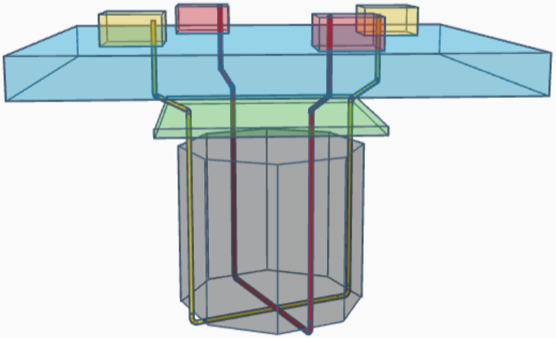
\includegraphics[width=\textwidth]{./Figures/Calibration-OverallSystemDesign.png}
\caption[Schematic of the sources insertion system]{Schematic representation of the system of guide tubes for insertion of sources.}
\label{fig:Calibration-OverallSystemDesign}
\end{figure}


%---
\subsection{Neutron Sources}

Neutron sources are of particular interest for calibration of the nuclear recoil PSD band and the efficiency of the neutron veto, a key feature of the \DSks\ design.  Small \alphan\ sources such as \AmBe\ and \AmC\ will be fabricated for this purpose. \AmBe\ is utilized as a tagged neutron source utilizing \AmBeGammaEnergy\ gamma in \AmTwoFourOneGammaTwoBR\ cases. \AmC\ can serve as a gamma-free source for Veto neutron calibration, after slowing down alphas for \alphan\ reaction to always produce daughters in the ground state. Sources will be small in size to be delivered with the source guide. 

While the \AmC\ source represents the best choice for calibration of the neutron detection efficiency, interactions in the source holder and materials between the source and the \TPC\ produced significant electron recoil background in the \DSfs\ \TPC, problematic for characterization of the nuclear recoils of argon nuclei. The \AmBe\ source was shown to be more suitable for this calibration. The \AmBeGammaEnergy\ \gr\ is promptly emitted in the \ce{^9Be}($\alpha$,n)\ce{^12C} nuclear reaction in about \SI{56}{\percent} of cases. By tagging the \AmBeGammaEnergy\ \gr\ in the Veto in a very tightly constrained time interval prior to the signal in the TPC, a very pure sample of nuclear recoils is obtained. The \AmBe\ calibration in \DSfs\ provided the best available nuclear recoil calibration of the \DSfs\ \TPC\ {\it in situ}, and was in excellent agreement with the nuclear recoil calibration from the stand-alone SCENE experiment~\cite{Cao:2015ks}.

The main novelty planned for the \AmBe\ calibration is a custom production of a miniature (a few \SI{}{\milli\meter}) \AmBe\ source, since the typically available commercial sources cannot fit within the planned narrow guide tube system. The miniature \AmBe\ source will rely on the procedure developed by the neutrino group at the University of Alabama~\cite{Ostrovkskiy:2012wv}. The group successfully fabricated an \AmBe\ source with an outer capsule dimension of just \CalAmBeSourceDiameter\ in diameter and \CalAmBeSourceLength\ long, with an activity of \CalAmBeSourceNeutronYield~neutrons per second using \CalAmBeAmSourceAmActivity\ of \ce{^241Am}. Fig.~\ref{fig:Cal-AmBeMiniatureUA} shows the outer and inner source capsules. The inner capsule is made of tungsten to efficiently suppress the \CalAmCSourceGammasEnergy\ gamma emission from the \ce{^241Am}. A very pure \ce{Be} powder is mixed with \ce{^241Am} high purity powder in an alcohol solution in a miniature test tube with a special micropipette and then transferred into the tungsten capsule. After the alcohol evaporates, the procedure is repeated. In the end, the mixture of \AmBe\ is compressed with a wire for higher source activity. The wire is also used to seal the tungsten capsule. The tungsten capsule is placed inside the stainless steel capsule and welded shut.  The source is then ready for certification and use. The outside capsule has a threaded part to attach the source to the rest of the calibration system.

\begin{figure}[!t]
\centering
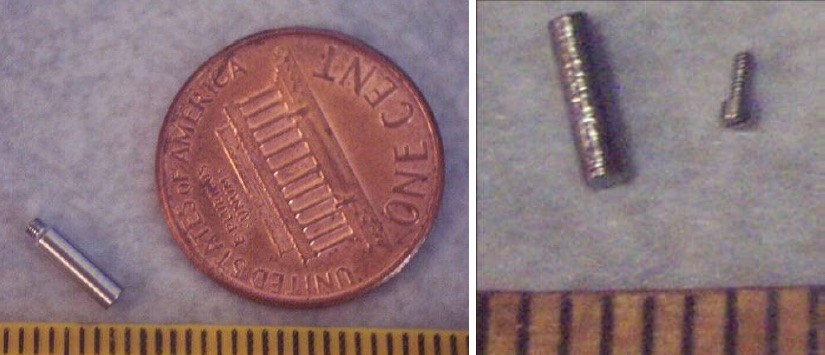
\includegraphics[width=\columnwidth]{./Figures/Cal-AmBeMiniatureUA.jpg}
\caption[Pictures of the miniature \AmBe\ neutron source]{{\bf Left:} the outer capsule of the custom made \AmBe\ source from the Alabama group~\cite{Ostrovkskiy:2012wv}.  {\bf Right:} the inner tungsten capsule of said \AmBe\ source.}
\label{fig:Cal-AmBeMiniatureUA}
\end{figure}

Photoneutron sources such as \YBe\ emit nearly monoenergetic \YBeNeutronEnergy\ neutrons, suitable for the low energy end of the nuclear recoil band. However, such source requires \TungstenShieldThickness\ thick tungsten shield to block copious \grs\ present in the source. Thus, this source is very bulky and requires a separate deployment system. Deployments will be monitored via a camera system to avoid any undesirable contact while operating in a delicate Veto.


%---
\subsection{Guide Tube System}

Implementation of calibration sources is being finalized, following the completion of the designs of the \TPC\, the Veto, and the \AAr\ cryostat. In parallel, plans are being developed for the calibration needs of the \DSks\ prototype detectors for x-y positioning, light yield and nuclear recoil calibration. While work is still in progress, the overall schematic of how to guide radioactive sources from the roof of the \AAr\ cryostat, down around and inside of the Veto detector, and then back up to the cryostat roof, is shown in Figure~\ref{fig:Calibration-OverallSystemDesign}.  The guide tube systems have been designed for simple, safe and efficient calibration of the Veto and \TPC\ using miniature radioactive sources. They will allow deployment of the sources inside the Veto without direct contact with the argon, eliminating risks associated with it. 

The guide tube system will bring radioactive sources from the top of the \AAr\ cryostat, to locations along the \TPC\ exterior. The sources will be delivered through an enclosed stainless steel tube coming vertically down from the top of the cryostat, passing by the \TPC\ \PMMA\ vessel and around its bottom. The guide tubes will be \CalGuideTubeDiameter\ (\CalGuideTubeDiameterInches) in diameter to minimize shadowing, dead space and radioactive background coming from the stainless steel. The stainless steel tube segments will be connected with Swagelok connectors. In addition, relatively small tube diameter will help for tighter control of the source location, especially important in the case of the gamma sources. 

The miniature sources will be attached to the stainless steel guide wire that will be pushed with a wire driver powered by a stepper motor. A sleeve, made out of the PTFE tubing, will envelope the guide wire and the source to significantly reduce friction while the source and its guide wire are being pushed around. The wire driver will be equipped with a set of encoders and two sensor boxes for accurate positioning of the source. A pair of ring type inductive proximity sensors placed inside the sensor box will be used to reset the encoders when sources pass through a sensor at exactly known locations. The system will be purged with a low pressure nitrogen to eliminate any residual radioactivity that may have entered into the tubes.

Except for the sensor box, all other parts of the guide tube system that require power, control and nitrogen flow will be at the top of the \AAr\ cryostat.  An elaborate testing program must be performed to ensure high quality and safety of the calibration when using the guide tube system. All parts will be radio-assayed and the entire system will be tested off-site for robustness, precision and reliability. Dedicated survey is planned to record the exact guide tube path around the \TPC\ \PMMA\ vessel.